


\tikzset{every picture/.style={line width=0.75pt}} %set default line width to 0.75pt        

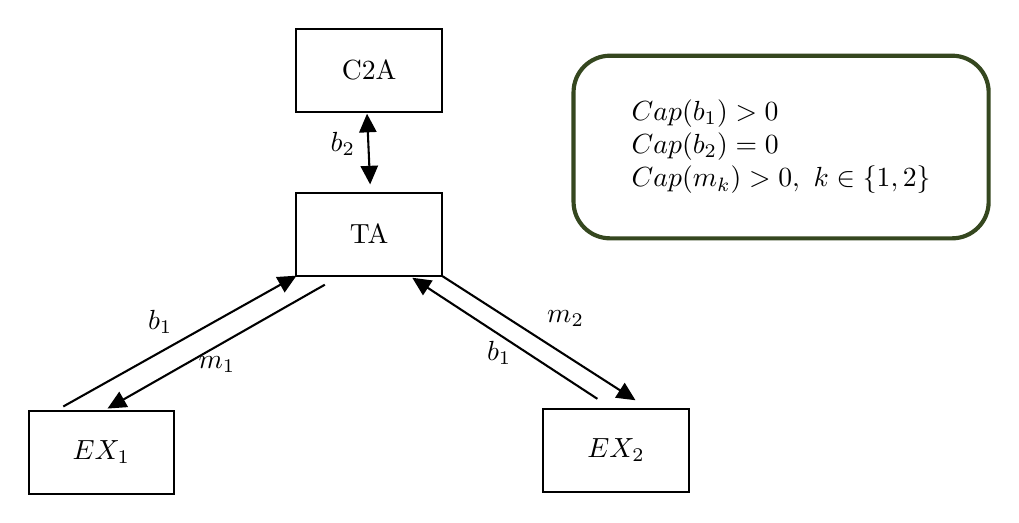
\begin{tikzpicture}[x=0.75pt,y=0.75pt,yscale=-1,xscale=1]
%uncomment if require: \path (0,268); %set diagram left start at 0, and has height of 268

%Shape: Rectangle [id:dp7793135649662085] 
\draw   (158,110) -- (228,110) -- (228,150) -- (158,150) -- cycle ;
%Shape: Rectangle [id:dp8388066725390221] 
\draw   (158,31) -- (228,31) -- (228,71) -- (158,71) -- cycle ;
%Shape: Rectangle [id:dp48691256180587716] 
\draw   (277,214) -- (347,214) -- (347,254) -- (277,254) -- cycle ;
%Shape: Rectangle [id:dp8836932328283702] 
\draw   (29,215) -- (99,215) -- (99,255) -- (29,255) -- cycle ;
%Straight Lines [id:da3337977868298102] 
\draw    (192.09,74) -- (193.41,104) ;
\draw [shift={(193.5,106)}, rotate = 267.47] [fill={rgb, 255:red, 0; green, 0; blue, 0 }  ][line width=0.75]  [draw opacity=0] (8.93,-4.29) -- (0,0) -- (8.93,4.29) -- cycle    ;
\draw [shift={(192,72)}, rotate = 87.47] [fill={rgb, 255:red, 0; green, 0; blue, 0 }  ][line width=0.75]  [draw opacity=0] (8.93,-4.29) -- (0,0) -- (8.93,4.29) -- cycle    ;
%Straight Lines [id:da7136052167478543] 
\draw    (171.67,154.33) -- (68.74,213.01) ;
\draw [shift={(67,214)}, rotate = 330.31] [fill={rgb, 255:red, 0; green, 0; blue, 0 }  ][line width=0.75]  [draw opacity=0] (8.93,-4.29) -- (0,0) -- (8.93,4.29) -- cycle    ;

%Straight Lines [id:da5349782032446363] 
\draw    (228,150) -- (319.65,208.92) ;
\draw [shift={(321.33,210)}, rotate = 212.74] [fill={rgb, 255:red, 0; green, 0; blue, 0 }  ][line width=0.75]  [draw opacity=0] (8.93,-4.29) -- (0,0) -- (8.93,4.29) -- cycle    ;

%Straight Lines [id:da1199439366931846] 
\draw    (45.67,213) -- (156.26,150.98) ;
\draw [shift={(158,150)}, rotate = 510.71] [fill={rgb, 255:red, 0; green, 0; blue, 0 }  ][line width=0.75]  [draw opacity=0] (8.93,-4.29) -- (0,0) -- (8.93,4.29) -- cycle    ;

%Straight Lines [id:da14294220152856596] 
\draw    (303,209.33) -- (215.51,152.09) ;
\draw [shift={(213.83,151)}, rotate = 393.19] [fill={rgb, 255:red, 0; green, 0; blue, 0 }  ][line width=0.75]  [draw opacity=0] (8.93,-4.29) -- (0,0) -- (8.93,4.29) -- cycle    ;

%Rounded Rect [id:dp3574279176331121] 
\draw  [color={rgb, 255:red, 53; green, 71; blue, 31 }  ,draw opacity=1 ][line width=1.5]  (291.5,61.6) .. controls (291.5,51.88) and (299.38,44) .. (309.1,44) -- (473.9,44) .. controls (483.62,44) and (491.5,51.88) .. (491.5,61.6) -- (491.5,114.4) .. controls (491.5,124.12) and (483.62,132) .. (473.9,132) -- (309.1,132) .. controls (299.38,132) and (291.5,124.12) .. (291.5,114.4) -- cycle ;

% Text Node
\draw (193,51) node  [align=left] {C2A};
% Text Node
\draw (193,130) node  [align=left] {TA};
% Text Node
\draw (64,235) node   {$EX_{1}$};
% Text Node
\draw (312,234) node   {$EX_{2}$};
% Text Node
\draw (92.33,172.33) node   {$b_{1}$};
% Text Node
\draw (255.67,187.33) node   {$b_{1}$};
% Text Node
\draw (119.67,193) node   {$m_{1}$};
% Text Node
\draw (287.67,170.67) node   {$m_{2}$};
% Text Node
\draw (180.33,86.33) node   {$b_{2}$};
% Text Node
\draw (391.5,88) node   {$ \begin{array}{l}
Cap( b_{1})  >0\\
Cap( b_{2}) =0\\
Cap( m_{k})  >0,\ k\in \{1,2\}
\end{array}$};


\end{tikzpicture}